\textbf{COLUNI 2025 -- Questão 21}\par\medskip Leia os textos a seguir.

\textbf{Texto I}

\begin{center}\textbf{These facts show how unsustainable the fashion industry is}\hfill\textbf{Jan 31, 2020}\end{center}

Some parts of modern life are, at this point, widely known to cause environmental harm -- flying overseas, using disposable plastic items, and even when we are driving to and from work, for example. But when it comes to our clothes, the impacts are less obvious. Fashion production makes up 10\% of humanity’s carbon emissions, dries up water sources, and pollutes rivers and streams. What’s more, 85\% of all textiles go to the dump each year. And washing some types of clothes sends thousands of bits of plastic into the ocean. Here are the most significant impacts fast fashion has on the planet.

Clothing production has roughly doubled since 2000. In Europe, fashion companies went from an average offering of two collections per year in 2000 to five in 2011. Some brands offer even more. Zara puts out 24 collections per year, while H\&M offers between 12 and 16. A lot of this clothing ends up in the dump. The equivalent of one garbage truck full of clothes is burned or dumped in a landfill every second. In total, up to 85\% of textiles go into landfills each year.

\noindent\begin{minipage}[t]{0.48\linewidth}\centering
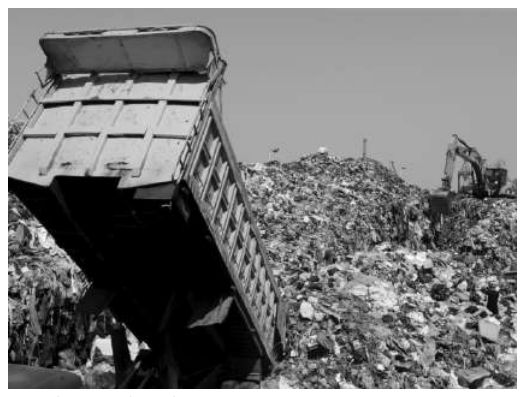
\includegraphics[width=\linewidth]{static/simulados/coluni/figuras/2025/questao-20/figura-1.png}\\
Landfill sites full of clothes all across the world. Image: REUTERS/Mohamed Azakir
\end{minipage}\hfill\begin{minipage}[t]{0.48\linewidth}\centering
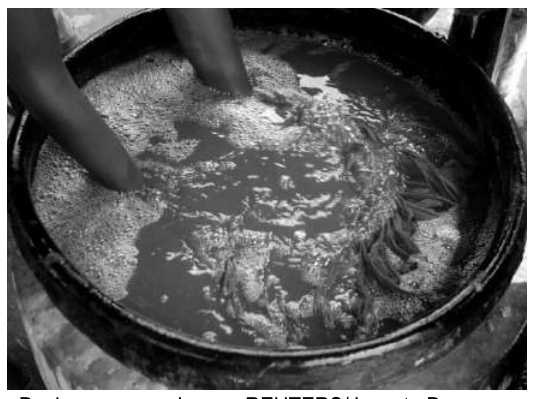
\includegraphics[width=\linewidth]{static/simulados/coluni/figuras/2025/questao-20/figura-2.png}\\
Dyeing process. Image: REUTERS/Jayanta Dey
\end{minipage}

Washing clothes, meanwhile, releases 500,000 tons of microfibers into the ocean each year -- the equivalent of 50 billion plastic bottles. Many of those fibers are polyester, a plastic found in an estimated 60\% of garments. Producing polyester releases two to three times more carbon emissions than cotton, and polyester does not break down in the ocean.

The fashion industry is responsible for 10\% of humanity’s carbon emissions. That’s more emissions than all international flights and maritime shipping combined. If the fashion sector continues on its current trajectory, that share of the carbon budget could jump to 26\% by 2050, according to a 2017 report from the Ellen MacArthur Foundation.

The fashion industry is also the second-largest consumer of water worldwide. It takes about 3,000 liters of water to produce one cotton shirt. That’s enough water for one person to drink at least eight cups per day for three-and-a-half years. It takes about 10,000 liters of water to produce a pair of jeans. That’s more than enough for one person to drink eight cups per day for ten years. That’s because both the jeans and the shirt are made from a highly water-intensive plant: cotton.

Fashion causes water-pollution problems, too. Textile dyeing is the world’s second-largest polluter of water, since the water leftover from the dyeing process is often dumped into ditches, streams, or rivers. The dyeing process uses enough water to fill 2 million Olympic-sized swimming pools each year. All in all, the fashion industry is responsible for 20\% of all industrial water pollution worldwide.

Some clothing companies are starting to buck these trends by joining initiatives to cut back on textile pollution and grow cotton more sustainably. In March, the UN launched the Alliance for Sustainable Fashion, which will coordinate efforts across agencies to make the industry less harmful.

\noindent Disponível em: https://www.weforum.org/agenda/2020/01/fashion-industry-carbon-unsustainable-environment-pollution/. Acesso em: 4 ago. 2024. (Adaptado)

\textbf{Texto II}

% COLUNI-AUTO-FIGURES-BEGIN
\begin{figure}[htbp]
\centering
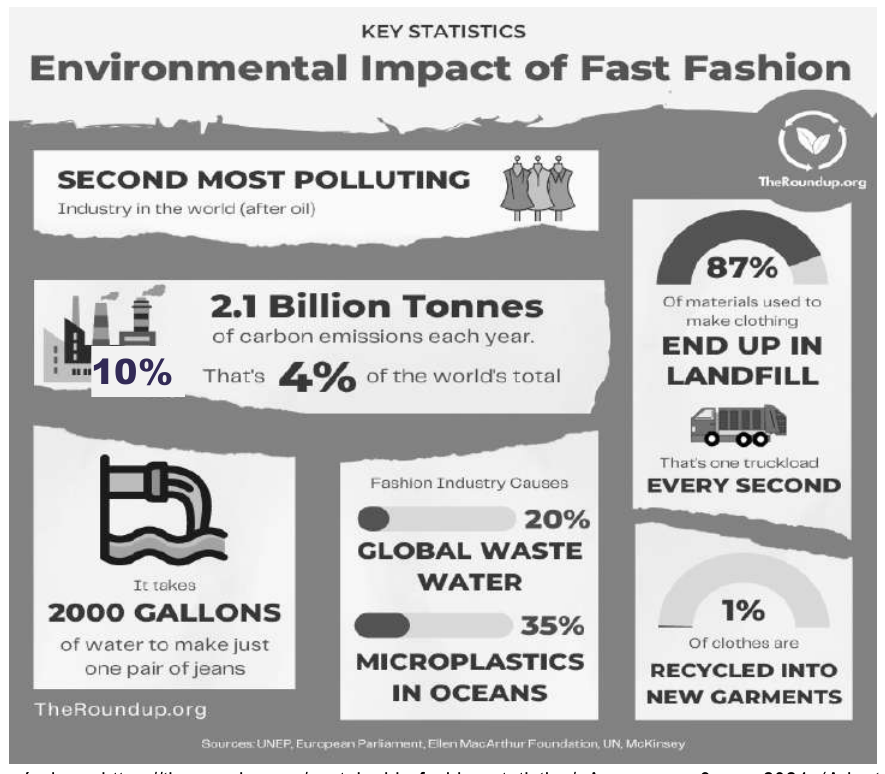
\includegraphics[width=0.78\linewidth]{static/simulados/coluni/figuras/2025/questao-21/figura-1.png}
\end{figure}
% COLUNI-AUTO-FIGURES-END
\noindent Disponível em: https://theroundup.org/sustainable-fashion-statistics/. Acesso em: 9 ago. 2024. (Adaptado)

Considerando as informações apresentadas nos textos I e II, é CORRETO afirmar que:
\begin{enumerate}
\item A água gasta na produção de uma calça jeans equivale à quantidade suficiente para uma pessoa beber oito copos de água por dia, durante três anos e meio.
\item A relação entre os dois textos é de contraste, pois as informações apresentadas no Texto II divergem-se das informações abordadas no Texto I.
\item Mais de 80\% das roupas produzidas pelas grandes marcas são queimadas ou descartadas todos os anos e apenas um por cento da produção é reciclada.
\item A indústria da moda é a segunda mais poluente do mundo, ficando atrás apenas da indústria petrolífera, emitindo menos carbono do que todos os voos internacionais e transporte marítimo juntos.
\end{enumerate}
